\htwo{Node.js}
\label{sec:nodejs}
\sectionauthor{Mersed Kečo}
Node.js ist eine plattformübergreifende JavaScript-Laufzeitumgebung, die auf der V8 JS-Engine von Google basiert. Node.js wurde entwickelt, um skalierbare Netzwerkanwendungen zu erstellen. Node.js ist beeinflusst von Ruby's "Event Machine" und Pythons "Twisted" und ähnelt diesen im Design. Die aktuelle Node.js-Version ist die Version 17, während die Veröffentlichung der Version 18 für den 25. Oktober 2022 geplant ist. Laut W3Techs wird Node.Js von 1,2\% aller Webseiten genutzt. Auf das ganze Internet gerechnet sind das über 20 Millionen Webseiten, die mithilfe von Node.js betrieben werden. \cite{Node}

\hfour{Die Architektur von Node.js}
Die von Node.js verwendete Architektur der "Single Threaded Event Loop" wird dazu verwendet, mehrere Clients gleichzeitig handzuhaben. Um überhaupt dem Unterschied zwischen dieser und anderen Runtimes auf die Spuren zu kommen, ist es von oberster Priorität zu verstehen, wie Multithreaded Concurrent Clients in Java gehandhabt werden. \cite{NodeJs.dev}


Das Modell des "Multithreaded Request/Response" versendet Anfragen an verschiedene Clients, worauf der Server jede einzelne verarbeitet, bevor er darauf eine Antwort versendet. Das Problem liegt aber jedoch daran, dass mehrere Threads verwendet werden, um gleichzeitige Aufrufe zu verarbeiten. Verwendete Threads sind in einem Thread-Pool definiert und werden einkommenden Anfragen zugewiesen, um diese zu bearbeiten. \cite{Arocom}



\begin{figure}[H]
    \centering
    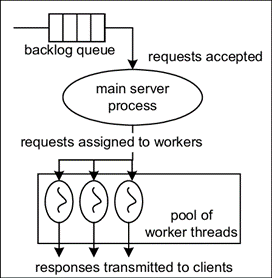
\includegraphics{media/NodeJs/MultiThreadedRequestResponse.png}
    \caption{Multithreaded Request/Response\cite{Multithreaded}}
\end{figure}

Thread-basierte Netzwerke sind ineffizient und äußerst schwierig zu verwenden. Node.js-Benutzer müssen sich keine Sorgen machen, dass ein Prozess blockiert wird, da es keine Sperren gibt. Es gibt kaum Möglichkeiten, einen Prozess zu sperren, außer wenn die E/A mit synchronen Methoden der Node.js-Standardbibliothek durchgeführt wird. Aufgrund des "not locking" Mechanismus sind skalierbare Systeme mit Node.js sehr einfach zu entwickeln. 
Node.js arbeitet mit dem Modell der "Event Loop", welches natürlich seine eigenen Vor- und Nachteile mitbringt und diese mit dem folgenden Beispiel schrittweise erläutert werden.


\begin{figure}[H]
    \centering
    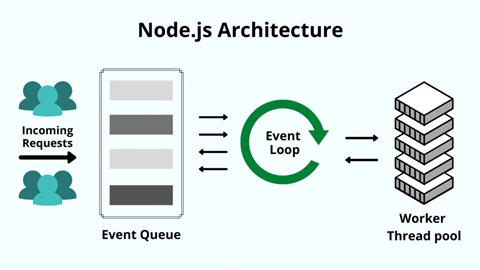
\includegraphics{media/NodeJs/NodeJsArchitektur.png}
    \caption{Node.Js Architektur\cite{ArchitekturFoto}}
\end{figure}


Node.js erlaubt nur eine begrenzte Anzahl an Threads in dem Threadpool, welche Anfragen bearbeiten.

Sobald Anfragen reinkommen, werden diese von Node.js in eine Warteschlange namens "Event Queue" eingeordnet. 

Die Kernkomponente der Architektur kommt an diesem Punkt zum Einsatz – die single threaded "Event Loop". Dieser Thread wartet auf unbestimmte Zeit auf eingehende Anfragen.

Bei einer eingehenden Anfrage holt die Loop diese aus der Queue und prüft, ob diese eine blockierende E/A-Operation benötigt. Falls dies nicht der Fall ist, wird die Anfrage verarbeitet und eine Antwort auf diese gesendet. 

Wenn die eingehende Anfrage aber eine blockierende E/O-Operation benötigt, verweist die "Event Loop" auf einen internen Thread aus seinem Threadpool, um diese Anfrage zu bearbeiten. Die Gruppe von Threads, die in solchen Situationen einspringen, wird Workergroup genannt.

Die Schleife verfolgt blockierende Anfragen und stellt solche in die Warteschlange. Jene Anfrage wird abgearbeitet, sobald davor auftretende blockierende Operationen abgearbeitet sind. Dies ist die Art und Weise, wie der Lebenszyklus von Nodes.js auf dem Laufenden gehalten werden kann.

Aufgrund der Verwendung von einer kleineren Anzahl von Threads, werden weniger Ressourcen beziehungsweise weniger Speicher verbraucht, welches sich auf die schnellere Ausführung von Anfragen ausübt. Wenn datenintensive Aufgaben verarbeitet werden müssen, dann ist die Verwendung von Multi-Threaded-Sprachen wie Java sinnvoller. In unserem Fall ist aber die Verwendung von Node.js die sinnvollste Wahl. \cite{Arocom}

\hfour{Anwendungen von Node.js}

Obwohl Node.js für eine Vielzahl von Anwendungen verwendet wird, sind einige Anwendungsfälle sehr beliebt und Node.js eine sehr gute Wahl dafür.

\begin{figure}[H]
    \centering
    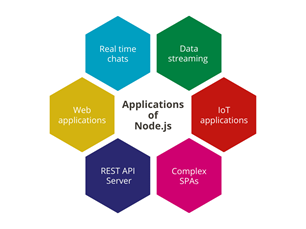
\includegraphics{media/NodeJs/NodeJsAnwendungen.png}
    \caption{Node.js Anwendungen \cite{AnwendungenFoto}}
\end{figure}

\begin{enumerate}
    \item Chats in Echtzeit
    \newline Die Node.js Architektur bietet eine gute Basis, um Echtzeit-Kommunikation zu verarbeiten. Durch die leichte Skalierbarkeit wird die Laufzeitumgebung oft bei der Entwicklung von Chatbots verwendet. Des Weiteren wird es einem Entwickler leicht gemacht, zusätzliche Chat-Funktionen wie Multi-Person-Chats und Push-Benachrichtigungen zu erstellen.
    \item Internet of Things
    \newline
    IoT-Anwendungen bestehen in den meisten Fällen aus mehreren Sensoren, die oftmals häufig, kleine Datenpakete senden, die sich mit der Zeit zu einer großen Anzahl von Anfragen anhäufen können. Node.js eignet sich aufgrund der schnellen, gleichzeitigen Verarbeitung von Anfragen dafür umso mehr.
    \item Komplexe Single-Page-Anwendungen (SPAs)
    \newline
    Bei SPAs wird die ganze Anwendung in einer Seite geladen. In der Regel bedeutet das, dass im Hintergrund gewisse Anfragen für bestimmte Komponenten gestellt werden. Die Eventschleife spielt in diesem Fall eine große Bedeutung.
    \item REST API-basierte Anwendungen
    \newline
    JavaScript wird nicht nur im Frontend, sondern auch im Backend von Webseiten eingesetzt. Mithilfe von Node.js besitzt ein Server somit die Möglichkeit, über REST APIs mit dem Frontend zu kommunizieren. Erwähnenswert ist noch, dass über Node.js bestimmte Pakete wie zum Beispiel Express.js zur Verfügung gestellt wird, die es noch einfacher machen, Webanwendungen zu erstellen.
    \item Daten-Streaming
    \newline
    Bekannte Unternehmen wie Netflix und Disney+ nutzen Node.js für Streaming-Zwecke. Der Grund dafür ist der, dass die Laufzeitumgebung schnell und leichtgewichtig ist. Wichtig zu erwähnen ist, dass eine native Streaming-API in Node.js schon vorweg implementiert ist. Streams ermöglichen den Nutzern, Anfragen aneinander weiterzuleiten, was das Ergebnis mit sich bringt, dass die Daten direkt an ihr Ziel gestreamt werden.
    
   \end{enumerate}
\cite{Anwendungen}



\hfour{Hello World in Node.js}

Um in die neu entdeckte Programmiersprache reinzuwachsen ist es oft so, dass man bei jeder neuen Programmiersprache ein "Hello World"-Programm schreibt. Dies sieht bei Node.js folgendermaßen aus:

\typescript{code/NodeJs/HelloWorld.ts}{HelloWorld in Node.js}

In unserem Codebeispiel wird das http Modul als erstes geladen. Danach wird die Methode "createServer" aufgerufen, um eine Anfrage anzunehmen und eine Antwort mit einem Statuscode zurückgibt. Letztendlich wird auf einen Port, der vordefiniert ist, gehört, ob Informationen an den Port gesendet werden.

Node.js wird den Entwicklern mit dem bereits eingebauten Modul namens "HTTP" bereitgestellt, welches ermöglicht, Daten über das "HyperText Transfer Protocol" (HTTP) zu übertragen. \cite{HelloWorld}

\hfour{NPM}
\label{sec:npm}

Der Node Package Manager (NPM) ist das Paket-System von Node.js. Es ist das größte Ökosystem aller Open Source Bibliotheken der Welt, mit über einer Millionen Pakete, weitere Pakete werden täglich releast. NPM ist kostenlos und hat eine sehr große Community, des öfteren Open Source Entwickler und begeisterte Programmierer. Die Firma, die hinter NPM steht, die sogenannte NPM INC. wurde 2014 gegründet und 2020 von GitHub aufgekauft.
NPM wird mit einem Kommandozeilenprogramm ausgeliefert. Die Möglichkeit besteht auch, auf der Webseite von NPM nach gewünschten Paketen zu suchen und diese mit einem einzigen Befehl zu installieren. Die Versionierung der Pakete und die Überprüfung von Abhängigkeiten kann eingerichtet werden. Node.js ist ein Dreh – und Angelpunkt für Entwickler vor allem wegen dem Package Support.
Die Sicherheit von Paketen ist bei NPM durch den bereits eingebauten Sicherheits-Scanner gegeben.

%TODO: Sicherheitslücken von NPM erwähnen, Bezugspunkt zu ZELIA(wie ist das Projekt aufgebaut, was verwenden wir)
\cite{NPM} \cite{NPM2}

\begin{figure}[H]
    \centering
    
\includegraphics{media/NodeJs/NPM.png}
    \caption{NPM Logo\cite{NPMLOGO}}
\end{figure}